\documentclass[10pt,x11names,table]{beamer}

\usetheme[progressbar=frametitle]{metropolis}
\usepackage{appendixnumberbeamer}
\usepackage{xcolor}

\usepackage{polyglossia}
\setmainlanguage{spanish}

\usepackage{listings}

\usepackage{booktabs}
\usepackage[scale=2]{ccicons}

\usepackage{pgfplots}
\usepgfplotslibrary{dateplot}

%ANIMACIONES
\usepackage{animate}
\usepackage{graphicx}
\usepackage[caption=false]{subfig}

\usepackage{xspace}

\newcommand*{\eg}{e.g.\@\xspace}
\newcommand*{\ie}{i.e.\@\xspace}

\let\oldquote\quote
\let\endoldquote\endquote
\renewenvironment{quote}[2][]
  {\if\relax\detokenize{#1}\relax
     \def\quoteauthor{#2}%
   \else
     \def\quoteauthor{#2~---~#1}%
   \fi
   \oldquote}
  {\par\nobreak\smallskip\hfill(\quoteauthor)%
   \endoldquote\addvspace{\bigskipamount}}
   
\usepackage{wrapfig}

\usepackage{subfig}
\usepackage{hyperref}
\usepackage{multicol}

\setbeamertemplate{bibliography item}[text]

\usepackage[font=small,skip=0pt, labelformat=empty]{caption}

\usepackage{dirtytalk}
\usepackage[acronym]{glossaries}
\makeglossaries

\newacronym{acgan}{ACGAN}{Auxiliary Classifier GAN}
\newacronym{ae}{AE}{Autoencoder}
\newacronym{ai}{AI}{Artificial Intelligence}
\newacronym{api}{API}{Application Programming Interface}
\newacronym{bert}{BERT}{Bidirectional Encoder Representations from Transformers}
\newacronym{brief}{BRIEF}{Binary Robust Independent Elementary Features}
\newacronym{brnn}{BRNN}{Bidirectional RNN}
\newacronym{bptt}{BPTT}{Backpropagation Through Time}
\newacronym{cbow}{CBOW}{Continous bag-of-words}
\newacronym{cnn}{CNN}{Convolutional Neural Network}
\newacronym{crnn}{CRNN}{Convolutional Recurrent Neural Network}
\newacronym{ddpm}{DDPM}{Denoising Diffusion Probabilistic Model}
\newacronym{ddim}{DDIM}{Denoising Diffusion Implicit Model}
\newacronym{diffit}{DiffiT}{Diffusion Vision Transformer}
\newacronym{dl}{DL}{Deep Learning}
\newacronym{dnn}{DNN}{Deep Neural Network}
\newacronym{dos}{DoS}{Denial of Service}
\newacronym{drnn}{DRNN}{Deep Recurrent Neural Network}
\newacronym{ecg}{ECG}{Electrocardiogram}
\newacronym{elmo}{ELMo}{Embedding from Language Model}
\newacronym{fast}{FAST}{Features from Accelerated Segment Test}
\newacronym{fid}{FID}{Fréchet Inception Distance}
\newacronym{foss}{FOSS}{Free and open-source software}
\newacronym{gan}{GAN}{Generative Adversarial Network}
\newacronym{glove}{GloVe}{Global Vectors for Word Representation}
\newacronym{gpu}{GPU}{Graphics Processing Unit}
\newacronym{gru}{GRU}{Gated Recurrent Unit}
\newacronym{ilsvrc}{ILSVRC}{ImageNet Large Scale Visual Recognition Challenge}
\newacronym{is}{IS}{Inception Score}
\newacronym{kid}{KID}{Kernel Inception Distance}
\newacronym{ldm}{LDM}{Latent Diffusion Model}
\newacronym{lstm}{LSTM}{Long Short-Term Memory}
\newacronym{mape}{MAPE}{Mean Absolute Perentage Error}
\newacronym{ml}{ML}{Machine Learning}
\newacronym{mlp}{MLP}{Multilayer Perceptron}
\newacronym{mmd}{MMD}{Maximum Mean Discrepancy}
\newacronym{mse}{MSE}{Mean Squared Error}
\newacronym{ner}{NER}{Named Entity Recognition}
\newacronym{nlg}{NLG}{Natural Language Generation}
\newacronym{nlp}{NLP}{Natural Language Processing}
\newacronym{nlu}{NLU}{Natural Language Understanding}
\newacronym{nn}{NN}{Neural Network}
\newacronym{ocr}{OCR}{Optical Character Recognition}
\newacronym{onnx}{ONNX}{Open Neural Network Exchange}
\newacronym{pmml}{PMML}{Predictive Model Markup Language}
\newacronym{relu}{ReLU}{Rectified Linear Unit}
\newacronym{rest}{REST}{Representational State Transfer}
\newacronym{rnn}{RNN}{Recurrent Neural Network}
\newacronym{sae}{SAE}{Stacked Autoencoder}
\newacronym{sift}{SIFT}{Scale-Invariant Feature Transform}
\newacronym{slam}{SLAM}{Simultaneous Localization and Mapping}
\newacronym{sru}{SRU}{Single Recurrent Unit}
\newacronym{surf}{SURF}{Speeded-Up Robust Features}
\newacronym{svm}{SVM}{Support Vector Machine}
\newacronym{vae}{VAE}{Variational Autoencoder}
\newacronym{vgg}{VGG}{Visual Geometry Group}
\newacronym{vit}{ViT}{Vision Transformer}
\newacronym{wsgi}{WSGI}{Web Server Gateway Interface}
\newacronym{xai}{XAI}{eXplainable Artificial Intelligence}
\newacronym{yolo}{YOLO}{You Only Look Once}
\newacronym{zsl}{ZSL}{Zero-shot Learning}
\subtitle{Métodos Generativos, curso 2024-2025}

\date{\today}
\author{Guillermo Iglesias, guillermo.iglesias@upm.es \newline
Jorge Dueñas Lerín, jorge.duenas.lerin@upm.es  \newline
Félix Fuentes Hurtado, felix.fuentes@upm.es}

\institute{Escuela Técnica Superior de Ingeniería de Sistemas Informáticos | UPM \newline
\hbox{} \newline \ccbysa \hspace{0.1pt} \ccNonCommercial}

%%%%%%%%%%%%%%%%%%%%%%%%%%%%%%%%%%%%%       
\title{Autoencoders}

\begin{document}
\maketitle


\begin{frame}{Contenidos}
  \begin{enumerate}
      \item Introducción
      \item Auto-encoders (AEs)
      \item{Auto-encoders Variacionales (VAEs)}
      \item{Generative Adversarial Networks (GANs)}
      \item{Transformers}
      \item{Diffusion Models}
    \end{enumerate}
\end{frame}


\begin{frame}{Contenidos}
  \begin{enumerate}
      \item Introducción
      \item \textbf{Auto-encoders (AEs)}
      \item{Auto-encoders Variacionales (VAEs)}
      \item{Generative Adversarial Networks (GANs)}
      \item{Transformers}
      \item{Diffusion Models}
    \end{enumerate}
\end{frame}

\section{Auto-encoders (AEs)}

\begin{frame}{¿Qué son los autoencoders?}
Un tipo de red neuronal que puede aprender a comprimir y luego reconstruir datos.

\begin{itemize}
    \item Un autoencoder es un tipo de red neuronal utilizada en tareas de aprendizaje no supervisado.
    \item Su objetivo es aprender una representación \textbf{compacta} de los datos de entrada.
    \item Consiste en dos partes principales: el codificador y el decodificador.
  \end{itemize}
\end{frame}

\begin{frame}{¿Qué son los autoencoders?}
Para operar, constan de dos componentes que se \textbf{entrenan al mismo tiempo}:

\begin{itemize}
    \item \textbf{Codificador}: Transforma los datos de entrada en una representación de menor dimensión.
    \item \textbf{Decodificador}: Toma esta representación y reconstruye los datos originales.
\end{itemize}

\begin{figure}
    \centering
    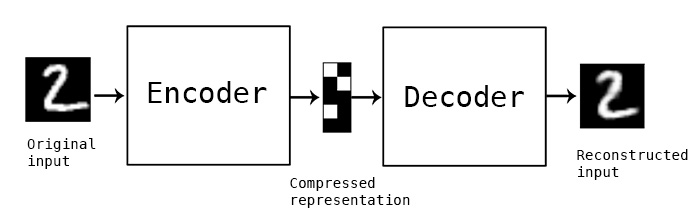
\includegraphics[width=.7\textwidth]{Slides/figures/02_Metodos_Generativos/cnn-ae.jpg}
    \caption{Estructura básica de un autoencoder.}
\end{figure}
\end{frame}

\begin{frame}{¿Para qué se emplean?}
Son muy útiles en una amplia variedad de aplicaciones.

\begin{itemize}
    \item Reducción de dimensionalidad de datos de alta dimensión.
    \item Eliminación de ruido en señales.
    \item Detección de anomalías.
    \item Generación de nuevos datos, similares a los datos de entrada\footnote{\href{https://scholar.google.es/citations?hl=es&user=iYN86KEAAAAJ}{Ian Goodfellow} menciona que son la \textbf{primera red generativa}.}.
\end{itemize}
\end{frame}


\begin{frame}{¿Cómo funcionan?}

A efectos prácticos, como cualquier otra red neuronal. Únicamente cambian la estructura del modelo, las entradas y salidas, y la función de pérdidas.

\begin{figure}
    \centering
    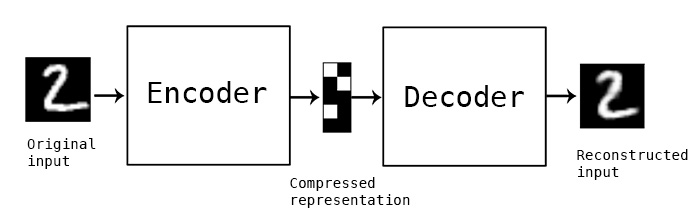
\includegraphics[width=.7\textwidth]{Slides/figures/02_Metodos_Generativos/cnn-ae.jpg}
\end{figure}

Su entrenamiento se realiza mediante el descenso de gradiente.

\begin{itemize}
    \item La \textbf{retropropagación} ajustará la salida de la red con respecto a la entrada.
    \item El entrenamiento tenderá a eliminar los datos que contribuyen menos a la salida, es decir, a encontrar una representación \textbf{comprimida} de los datos de entrada.
\end{itemize}
\end{frame}


\begin{frame}{¿Cómo funcionan?}

Un ejempo real de un autoencoder podría ser el siguiente:

\begin{figure}
    \centering
    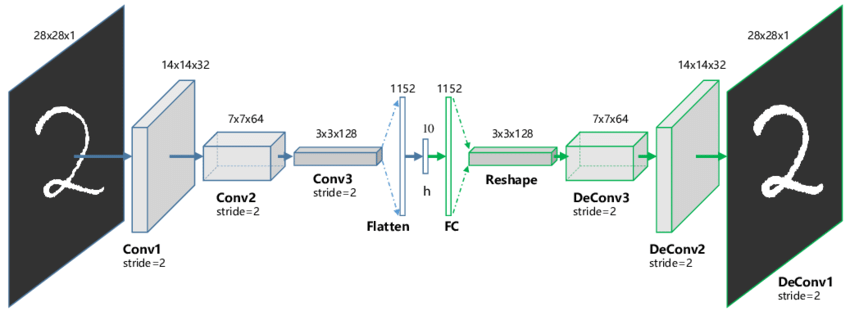
\includegraphics[width=\textwidth]{Slides/figures/02_Metodos_Generativos/2.2. ae conv.png}
    \caption{Esquema de un Autoencoder convolucional (\href{https://www.researchgate.net/profile/Xifeng-Guo/publication/320658590/figure/fig1/AS:614154637418504@1523437284408/The-structure-of-proposed-Convolutional-AutoEncoders-CAE-for-MNIST-In-the-middle-there.png}{fuente}).}
\end{figure}

\end{frame}

\begin{frame}{¿Cómo funcionan?}

\begin{figure}
    \centering
    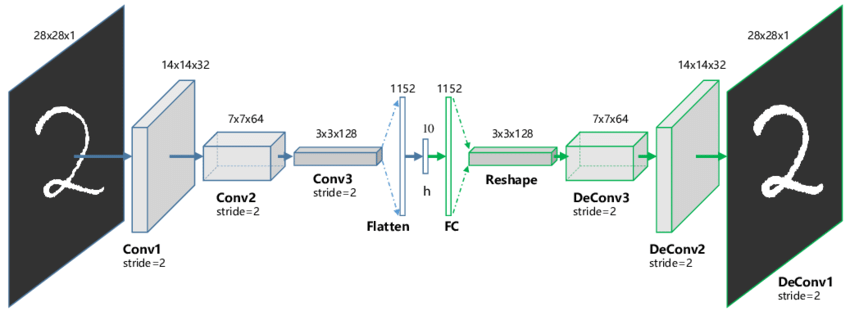
\includegraphics[width=.7\textwidth]{Slides/figures/02_Metodos_Generativos/cnn-ae-adv.png}
\end{figure}

Podemos observar que se compone de:
\begin{itemize}
    \item El codificador o \textit{\textbf{encoder}}: calcula una representación comprimida de los datos de entrada.
    \item El \textbf{\textit{bottleneck}}: la información que representa los datos de entrada de forma comprimida.
    \item El decodificador o \textit{\textbf{decoder}}: trata de reconstruir los datos de entrada a partir de la información del \textit{bottleneck}.
\end{itemize}
\end{frame}


\begin{frame}{¿Cómo se entrenan?}

Se entrenan de igual forma que las redes neuronales tradicionales.

La función de pérdidas suele ser parecida a la que se emplearía en problemas de \textbf{regresión}, pues, al final, se trata de eso mismo.

\begin{figure}
    \centering
    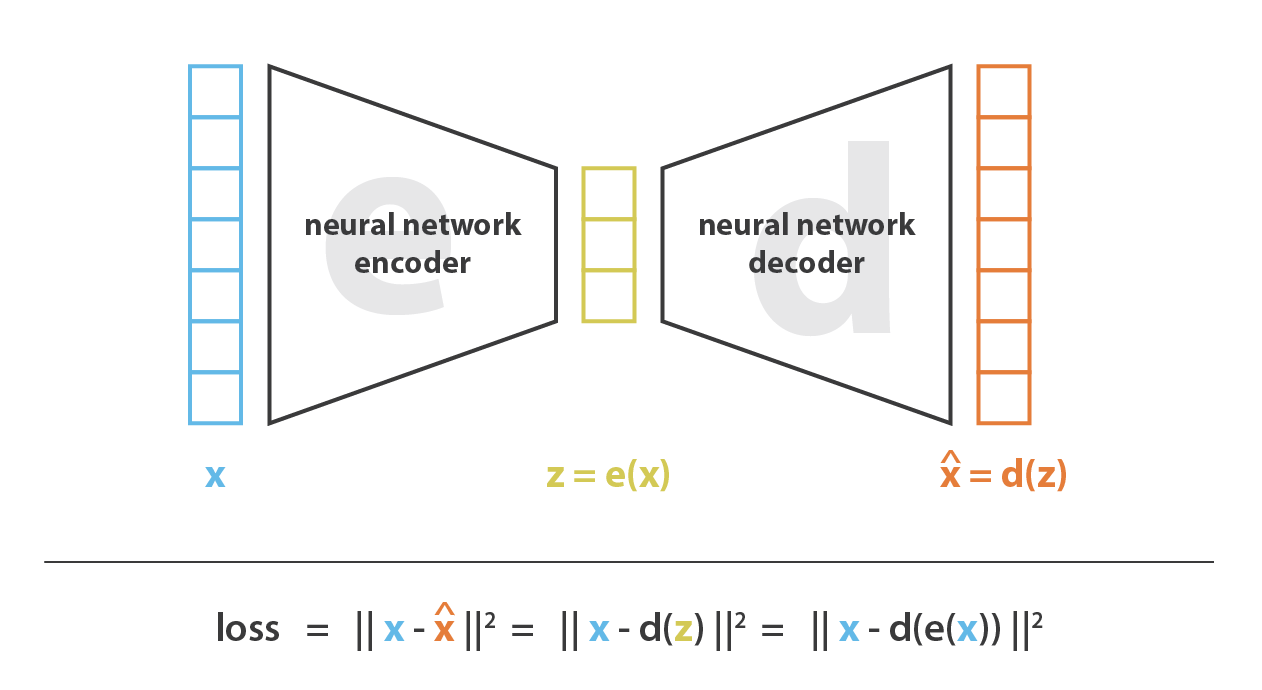
\includegraphics[width=.7\textwidth]{Slides/figures/02_Metodos_Generativos/cnn-ae-loss.png}
\end{figure}

Podemos observar que se compone de:
\begin{itemize}
    \item El codificador o \textit{\textbf{encoder}}: calcula una representación comprimida de los datos de entrada.
    \item El \textbf{\textit{bottleneck}}: la información que representa los datos de entrada de forma comprimida.
    \item El decodificador o \textit{\textbf{decoder}}: trata de reconstruir los datos de entrada a partir de la información del \textit{bottleneck}.
\end{itemize}
\end{frame}


\begin{frame}{¿Por qué necesitamos Autoencoders?}

Los autoencoders tienen muchas aplicaciones en el mundo real:

\begin{itemize}
    \item Compresión y reconstrucción de imágenes.
    \item Generación de música y separación de fuentes de sonido.
    \item Compresión de archivos para reducir el tamaño sin perder información importante.
    \item Extracción de características numéricas de señales de voz que se pueden usar para identificar palabras y frases.
    %\item Filtrado de spam.
\end{itemize}
\end{frame}


\begin{frame}{Tipos de autoencoders}

Los autoencoders son modelos que tienen muchas variaciones. Las más comunmente utilizadas son:

\begin{itemize}
    \item Vanilla Autoencoder
    \item Stacked autoencoders
    \item Denoising Autoencoder
    \item Convolutional Autoencoder
    \item \textit{Variational Autoencoder}\footnote{Los veremos más adelante, ya que introducen variaciones importantes en la arquitectura básica de un autoencoder.}
\end{itemize}

\end{frame}


\section{Vanilla Autoencoder}

\begin{frame}{Vanilla Autoencoder}

Son el tipo más simple de autoencoder.

\begin{itemize}
    \item Introducidos por Hinton y Salakhutdinov en su artículo ``\textit{Reducing the dimensionality of data with neural networks}''~\cite{hinton2006reducing}.
\end{itemize}

Consisten en una sola capa oculta.

\begin{itemize}
    \item Que se llama ``espacio latente'' y se denota como $z$
\end{itemize}

Son una forma simple y efectiva de aprender representaciones comprimidas de datos.

\begin{itemize}
    \item Se pueden usar para compresión de datos y reducción de dimensionalidad.
    \item Para otras aplicaciones, como generación de datos sintéticos, no son las mejores elecciones.
\end{itemize}
\end{frame}

\begin{exercise}
\href{https://colab.research.google.com/drive/1-YAytBp9L5nkHvAxKV7urjaeE6HH58Dj}{Comprimiendo datos con Vanilla Autoencoder}

% {\small
% \href{https://colab.research.google.com/drive/10QEVkfFtW3Dk0X_bazwTDMKaDBq4N08v}{(Solución)}
% }
\end{exercise}

\begin{frame}{Limitaciones de los Vanilla Autoencoder}
Los Vanilla Autoencoder no son muy eficientes en la generación de datos sintéticos.

\textbf{Problema principal}: El \textbf{espacio latente generado no es continuo}.

\begin{itemize}
    \item Está compuesto por regiones separadas entre sí que agrupan características de ejemplos similares.
    \item Entre estas regiones no hay un espacio continuo de representaciones intermedias.
    \begin{itemize}
        \item En realidad, lo hay, pero no tiene sentido.
        \item ¿Realmente no hay un espacio intermedio entre un 1 y un 7? ¿o entre un 3 y un 8?
    \end{itemize}
    \item Esto hace que la interpolación entre ejemplos sea imposible.
\end{itemize}

En resumen, \textbf{si el espacio intermedio no es continuo, las salidas del decodificador no son realistas}. --> Esto lo solucionan los autoencoders variacionales
\end{frame}


\section{Autoencoders Convolucionales}

\begin{frame}{Autoencoders Convolucionales}
Un tipo de red neuronal diseñado para procesar y reconstruir datos de imágenes.

\begin{itemize}
    \item Utilizan \glspl{cnn} debido a su capacidad para capturar relaciones espaciales entre píxeles.
    \item El codificador típicamente consta de varias capas convolucionales, seguidas de un conjunto de capas totalmente conectadas.
    \begin{itemize}
        \item Las capas convolucionales extraen características de la imagen de entrada.
        \item Las capas totalmente conectadas luego combinan estas características en una representación de menor dimensión de la imagen.
    \end{itemize}
    \item El decodificador es esencialmente un espejo del codificador, con un conjunto de capas totalmente conectadas seguidas de varias capas deconvolucionales.
\end{itemize}
\end{frame}

\begin{frame}{Autoencoders Convolucionales}

\begin{figure}
    \centering
    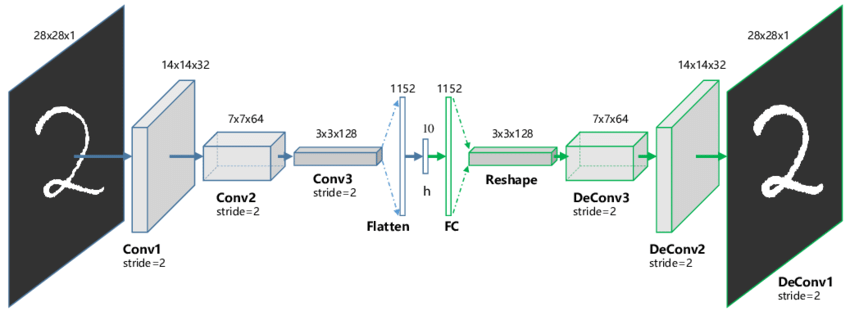
\includegraphics[width=0.8\textwidth]{Slides/figures/02_Metodos_Generativos/2.2. ae conv.png}
    \caption{Esquema de un Autoencoder convolucional (\href{https://www.researchgate.net/profile/Xifeng-Guo/publication/320658590/figure/fig1/AS:614154637418504@1523437284408/The-structure-of-proposed-Convolutional-AutoEncoders-CAE-for-MNIST-In-the-middle-there.png}{fuente}).}
\end{figure}

Pueden aprender a representar datos de imágenes de manera más compacta y eficiente

\begin{itemize}
    \item Reduciendo así la cantidad de memoria y potencia de procesamiento necesarias para tareas posteriores como clasificación de imágenes o detección de objetos.
\end{itemize}
\end{frame}


\begin{exercise}
\href{https://colab.research.google.com/drive/1p1F4vTvJ0FNQ-sJEibo22bEx5inPbMyL}{Autoencoders convolucionales}

% {\small
% \href{https://colab.research.google.com/drive/1VQ_P-FWUE1qanbKIyO-c6s1RrSDOnb0U}{(Solución)}
% }
\end{exercise}


\section{Autoencoders de Eliminación de Ruido (Denoising Autoencoders)}

\begin{frame}{Autoencoders de Eliminación de Ruido (Denoising Autoencoders)}

Son similares a un autoencoder vanilla~\cite{vincent2008extracting}:

\begin{itemize}
    \item La red típicamente consta de un codificador y un decodificador.
    \item La diferencia: una capa de ruido que agrega ruido a los datos de entrada.
    \item Agrega ruido a los datos de entrada antes de que se alimenten al codificador.
\end{itemize}

\end{frame}


\begin{frame}{Autoencoders de Eliminación de Ruido (Denoising Autoencoders)}
Durante el entrenamiento, se presentan pares de datos de entrada con ruido y datos de salida limpios.

\begin{itemize}
    \item La red se entrena para minimizar la diferencia entre los datos de entrada originales y los datos de salida reconstruidos, teniendo en cuenta el ruido añadido.
\end{itemize}

La capa de ruido se puede personalizar según el tipo de ruido:

\begin{itemize}
    \item \eg Ruido gaussiano: Capa que agrega ruido gaussiano a los datos de entrada.
    \item \eg Ruido sal y pimienta: Capa que establece algunos píxeles en cero.
\end{itemize}

\textbf{Pueden aprender representaciones \alert{robustas} de datos \alert{menos sensibles al ruido}}.
\end{frame}

\begin{exercise}
\href{https://colab.research.google.com/drive/1oRkjwRem9HBvq2557Lcc2ZsT-nR0qo30}{Supresión de ruido en imágenes con autoencoders de eliminación de ruido}

% {\small
% \href{https://colab.research.google.com/drive/1WIaSh2P-wl2mCQ0SAjeJk06pi-KWMj60}{(Solución)}
% }
\end{exercise}


\section{Autoencoders Apilados (Stacked autoencoders)}

\begin{frame}{\acrfullpl{sae}}
Tipo de red neuronal compuesta por múltiples capas de autoencoders~\cite{vincent2010stacked}.

\begin{itemize}
    \item Cada capa consta de un codificador y un decodificador, similar a un autoencoder vanilla.
    \item La salida de una capa se alimenta como entrada a la siguiente, creando una red neuronal profunda.
\end{itemize}

\begin{figure}
    \centering
    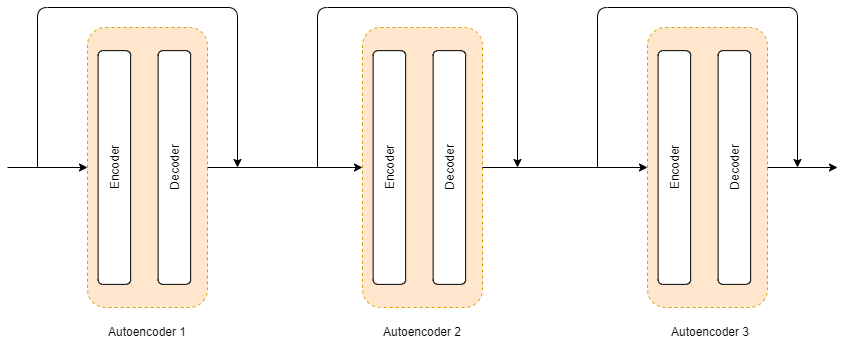
\includegraphics[width=.45\textwidth]{Slides/figures/02_Metodos_Generativos/nn-stack-autoencoder-1.png}
    \caption{Autoencoder apilado}
\end{figure}

Permiten una representación más poderosa de los datos que se puede utilizar en tareas posteriores.
\end{frame}

\begin{frame}{\acrshort{sae} como método de entrenamiento de redes neuronales profundas}

\begin{columns}
    \begin{column}{.4\linewidth}
        \begin{center}
        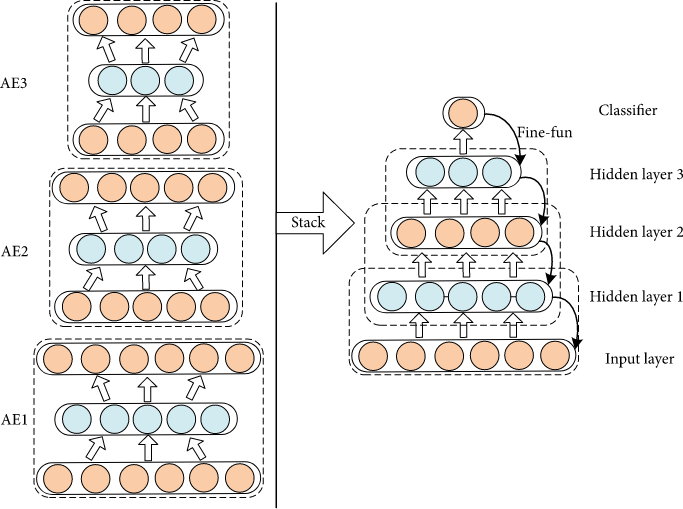
\includegraphics[width=\textwidth]{Slides/figures/02_Metodos_Generativos/nn-stack-autoencoder-2.png}
        \end{center}
    \end{column}
    \begin{column}{.6\linewidth}
        De hecho, los \acrshortpl{sae} pueden usarse como técnica para el entrenamiento de \acrshortpl{mlp}:

        \begin{enumerate}
            \item Cada capa del autoencoder apilado se entrena por separado para reconstruir sus datos de entrada.
            \item Una vez que una capa se entrena, su salida se usa como entrada para la siguiente capa.
            \item Cuando toda la red ha sido entrenada, los espacios latentes resultantes se apilan.
        \end{enumerate}
    \end{column}
\end{columns}
\vspace{1em}
Luego, se ajusta finamente la red resultante para minimizar el error de reconstrucción entre los datos de entrada originales y los datos de salida finales.

\begin{itemize}
    \item Esta fue una de las primeras técnicas para entrenar redes neuronales profundas~\cite{hinton2006reducing}.
\end{itemize}
\end{frame}

\begin{exercise}
\href{https://colab.research.google.com/drive/18_mDUr6XVRtWmUcJ7UuZgODjWblpAS2f}{Autoencoders apilados y la reconstrucción de fashion MNIST}
\end{exercise}

%%%%%%%%%%%%%%%%%%%%%%%%%%%%

\begin{frame}{Recursos}
\begin{itemize}
    \item Diapositivas de Moodle
    \item Google Collaboratory
    \item Deep Learning Book (https://www.deeplearningbook.org/)
    \item https://www.pyimagesearch.com/blog
    \item https://machinelearningmastery.com/blog
\end{itemize}
\end{frame}

% \section{Auto-encoders Variacionales (VAEs)}
% % \begin{frame}{Auto-encoders Variacionales(VAEs)}
% % \end{frame}

% \section{Generative Adversarial Networks (GANs)}
% % \begin{frame}{Generative Adversarial Networks (GANs)}
% % \end{frame}

% \section{Transformers}
% % \begin{frame}{Transformers}
% % \end{frame}

% \section{Diffusion Models}
% % \begin{frame}{Diffusion Models}
% % \end{frame}


\appendix

\begin{frame}[allowframebreaks]{Referencias}
    \bibliography{references}
    \bibliographystyle{abbrv}
\end{frame}

\begin{frame}<presentation:0>{License}
    \begin{block}{Tema \texttt{slides-upm}. Puedes obtener sus fuentes en}
        \begin{center}\url{http://gitlab.com/blazaid/slides-upm}\end{center}
    \end{block}
  
    Tanto esta presentación como el tema están licenciados bajo \href{http://creativecommons.org/licenses/by-sa/4.0/}{Creative Commons
  Atribución-CompartirIgual 4.0 Internacional (CC BY-SA 4.0)}.
    \begin{center}\ccbysa\end{center}
\end{frame}

\end{document}
